\subsection{Шкала электромагнитных волн}


\term{Гамма излучение} возникают при радиоактивных распадах ядер, при торможении электронов энергией более $10^5$~эВ и при других взаимодействиях элементарных частиц. Используются в гамма-дефектоскопии, при изучении свойств вещества.

\term{Рентгеновские лучи} излучаются при большом ускорении электронов, например их торможение в металлах. Получают при помощи рентгеновской трубки: электроны в вакуумной трубке ускоряются электрическим полем при высоком напряжении, достигая анода, при со­ударении резко тормозятся. При торможении электроны движут­ся с ускорением и излучают электромагнитные волны с малой длиной. 

\begin{figure}[!h]
\centering
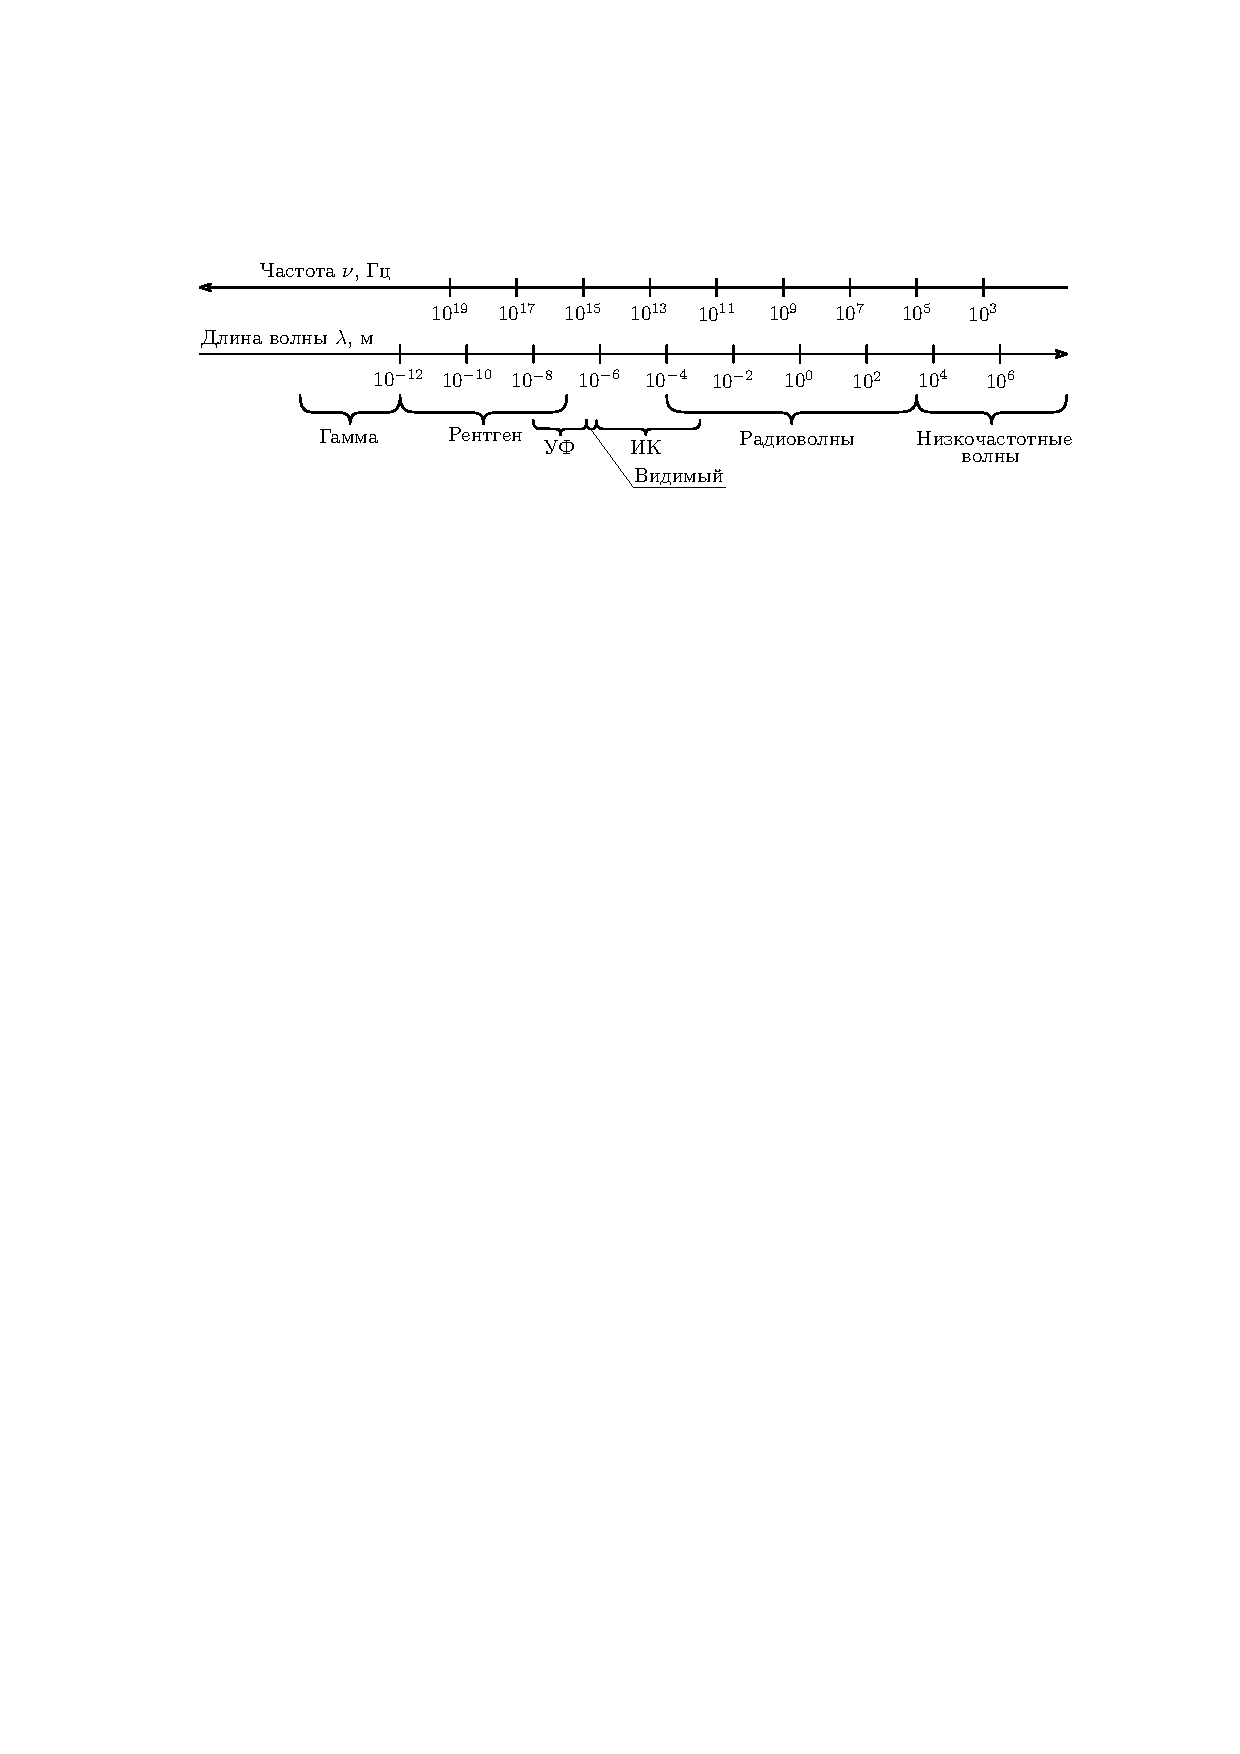
\includegraphics[width = 1\textwidth]{scale-wave.pdf}
\caption{Шкала электромагнитных волн}
\end{figure}
\term{Ультрафиолетовые лучи}~--- излучение Солнца, ртутных ламп и т.\,п. Используются в ультрафиолетовой микроскопии, в медицине.

\term{Видимое излучение}~--- часть электромагнитного излучения, воспринимаемая глазом (от фиолетового до от красного).

\term{Инфракрасное излучение}~--- тепловое, излучается любым нагретым телом.

\term{Радиоволны} используются повсеместно в обычной жизни, это и сотовая связь, и радиолокация, и спутниковая связь, и многое другое.

\term{Низкочастотные волны}~--- диапазон, традиционно используемый в электротехнике. В промышленной электроэнергетике используется частота 50~Гц, на~которой осуществляется передача электрической энергии по линиям и преобразование напряжений трансформаторными устройствами.